%File: main.tex  --  AAAI-26 anonymous submission
\documentclass[letterpaper]{article}
\usepackage[submission]{aaai2026}  % Keep [submission] for double-blind; remove for camera-ready
\usepackage{times}
\usepackage{helvet}
\usepackage{courier}
\usepackage[hyphens]{url}
\usepackage{graphicx}
\urlstyle{rm}
\def\UrlFont{\rm}
\usepackage{natbib}
\usepackage{caption}
\frenchspacing
\setlength{\pdfpagewidth}{8.5in}
\setlength{\pdfpageheight}{11in}
% Allowed technical packages:
\usepackage{amsmath,amssymb,amsthm}
\usepackage{booktabs}
\usepackage{algorithm}
\usepackage{algorithmic}
\usepackage{tikz}
\usetikzlibrary{positioning,arrows.meta,fit}

\pdfinfo{
/TemplateVersion (2026.1)
}

\setcounter{secnumdepth}{2}

\newtheorem{definition}{Definition}
\newtheorem{proposition}{Proposition}
\newtheorem{assumption}{Assumption}

% Notation macros -- single source of truth is notes/NOTATION.md
\newcommand{\V}{\mathcal{V}}            % vocabulary
\newcommand{\K}{\mathcal{K}}            % key space
\newcommand{\T}{\mathcal{T}}            % task set
\newcommand{\Sd}{\mathcal{S}}           % sampling-seed set
\newcommand{\G}{G}                      % green list
\newcommand{\Fn}{F}                     % functional outcome
\newcommand{\Sec}{S}                    % security outcome
\newcommand{\Y}{Y}                      % secure-and-functional outcome
\newcommand{\WM}{\mathrm{wm}}
\newcommand{\Base}{\varnothing}         % unwatermarked arm
\newcommand{\E}{\mathbb{E}}
\newcommand{\Var}{\operatorname{Var}}
\newcommand{\Cov}{\operatorname{Cov}}
\newcommand{\ATE}{\Delta}               % average KGW effect


% ---------------------------------------------------------------------------
% Candidate titles (Step 1). The active title is the first one.
%  (1) Are Valid Watermark Keys Interchangeable? A Paired Protocol and Pilot Evidence
%      for KGW-Watermarked Secure Code Generation                       <-- active
%  (2) Watermark Keys Are Not Free Parameters: Measuring Key Heterogeneity in
%      Secure Code Generation
%  (3) One Model, Ten Keys: A Pilot Audit of KGW Watermarking for Secure Code
%  (4) Separating Watermark Cost from Key Choice in LLM Code Generation
%  (5) Does the Watermark Key Matter? Paired Evaluation of KGW on Functional and
%      Secure Code
% ---------------------------------------------------------------------------
\title{Are Valid Watermark Keys Interchangeable? A Paired Protocol and Pilot Evidence for KGW-Watermarked Secure Code Generation}
\author{
    Anonymous Submission
}
\affiliations{
}

\begin{document}

\maketitle

\begin{abstract}
Statistical watermarks such as KGW bias a language model toward a keyed ``green'' subset of the vocabulary so that its outputs can later be attributed. Deployments treat the secret key as a free parameter: any valid key is assumed to be behaviorally interchangeable. For code generation this assumption is consequential, because a single token can separate a secure program from a vulnerable or broken one, yet evaluations of watermarked code use one key and measure correctness, not security. We formulate the question as two distinct estimands, the average effect of watermarking relative to matched unwatermarked generation and the between-key heterogeneity among valid keys, and give a paired, clustered measurement protocol with fail-closed manipulation gates. We show that between-key contrasts do not depend on the shared baseline, and derive a first-order output-length requirement for per-output detection. We then report pilot evidence for one open code model under a preregistered setting. A calibration of 7,200 generations shows a monotone dose response in detector strength. A ten-key pilot of 792 programs shows functional pass rates ranging from 12.5\% to 70.8\% across keys, while security labels are nearly key-invariant and only 2.9\% of watermarked outputs are individually detectable. We therefore do not claim a key-dependent security effect; we identify the validation gates that must pass before such a claim can be tested.
\end{abstract}

\section{Introduction}
\label{sec:intro}

Watermarking is one of the few mechanisms that lets a model provider later recognise text its model produced without storing every output. The most widely studied family, introduced by \citet{kirchenbauer2023watermark} and commonly called KGW, hashes a secret key together with the preceding token to pseudo-randomly select a ``green'' fraction $\gamma$ of the vocabulary, adds a bias $\delta$ to the logits of green tokens, and detects the watermark with a one-proportion $z$-test on the count of green tokens. Variants of this idea now ship in widely used open-source libraries \citep{wolf2020transformers,pan2024markllm} and are evaluated in dedicated benchmarks \citep{tu2024waterbench,piet2023markmywords}.

The key is treated as a free parameter. Because the partition is produced by a hash, any valid key is assumed to be as good as any other, and quality evaluations of watermarking typically report results for a single, fixed key. This assumption is plausible for prose, where many surface forms are acceptable. It is less obviously safe for code. A program's security can depend on a single token, such as \texttt{snprintf} versus \texttt{sprintf} or \texttt{yaml.safe\_load} versus \texttt{yaml.load}, and LLM-generated code is already frequently insecure without any watermark \citep{pearce2022asleep,bhatt2023cyberseceval,peng2025cweval}. For a fixed key and context, KGW applies the same deterministic preference every time that context recurs. If a key happens to place insecure idioms on the green side of recurring contexts, its bias could recur in many generated programs. Whether this happens is an empirical question that, to our knowledge, has not been tested for code security.

\paragraph{Two questions, not one.} Answering it requires separating two estimands that are easily conflated. The \emph{average effect} of KGW compares watermarked and matched unwatermarked generation and measures the price of watermarking. \emph{Between-key heterogeneity} compares valid keys with each other and tests the interchangeability assumption itself. A large spread between the best and worst of a few keys is not evidence of heterogeneity unless it exceeds what sampling noise and task clustering produce, and a heterogeneity claim is only meaningful if the watermark manipulation was actually applied and the security oracle can discriminate.

\paragraph{This paper.} We study a single open model, Qwen2.5-Coder-7B-Instruct \citep{hui2024qwen25coder}, with the KGW implementation in Hugging Face Transformers. Our evidence is preliminary and we report it as such. The pilot shows large key-associated variation in \emph{functional} correctness. It does not show key-dependent \emph{security}, and its detector diagnostics show that the watermark manipulation is not yet validated for short programs. We think these diagnostic and negative findings are useful in their own right: they show which validity threats a key-audit study has to rule out before any key can be called harmful.

\paragraph{Contributions.}
\begin{itemize}
\item \textbf{Formulation.} We define the average KGW effect and between-key heterogeneity as separate estimands over a paired task$\times$seed design. We prove that between-key contrasts are invariant to the shared unwatermarked baseline (Proposition~\ref{prop:baseline}) and derive a first-order minimum output length for per-output KGW detection (Proposition~\ref{prop:length}).
\item \textbf{Protocol and artifact.} We describe a fail-closed audit pipeline: deterministic key derivation, provenance-stamped resumable generation, a networkless sandbox for executing generated code, deterministic C/Python oracles over 12 CWE families, and preregistered manipulation and go/no-go gates.
\item \textbf{Pilot evidence.} A 7,200-generation calibration shows a monotone bias dose response. A 792-program ten-key pilot shows functional rates from 12.5\% to 70.8\% across keys, near-constant security labels, and weak per-output detection (21/720 outputs at $z\!\ge\!4$; five of ten keys with negative mean $z$).
\item \textbf{Validity analysis.} We list the threats that currently prevent a security claim and the concrete gates that address them, so that the planned 100-key study can produce a falsifiable result.
\end{itemize}

\section{Related Work}
\label{sec:related}

\subsection{Statistical Watermarks for Language Models}
KGW \citep{kirchenbauer2023watermark} partitions the vocabulary with a keyed hash of the preceding context and biases green logits. \citet{kirchenbauer2024reliability} study its robustness and introduce additional seeding schemes, including the self-hashing (``selfhash'') scheme used in this work. Unigram watermarking fixes a single global partition \citep{zhao2024provable}. Distortion-free schemes preserve the next-token distribution in expectation over keys \citep{kuditipudi2024robust,mao2025unbiased}, and SynthID-Text uses tournament sampling at production scale \citep{dathathri2024scalable}. \citet{fernandez2023threebricks} sharpen the statistical tests used for detection, and \citet{jovanovic2024stealing} show that the keyed rules can be estimated and spoofed through queries. Quality is usually evaluated on aggregate text benchmarks \citep{tu2024waterbench,piet2023markmywords}. Some text-domain work reports variation in perplexity across keys \citep{mao2025unbiased}. \emph{Contrast:} these works treat the key as a secret to protect or as a source of noise to average over. We treat key choice itself as a treatment whose effect on downstream program correctness and security has to be measured.

\subsection{Watermarking Generated Code}
Code has low-entropy stretches where any bias can break syntax. SWEET \citep{lee2024sweet} therefore watermarks only high-entropy tokens and reports that plain KGW reduces functional pass rates on code benchmarks. \citet{suresh2024robust} show that semantics-preserving transformations such as renaming remove code watermarks. \emph{Contrast:} these studies measure the \emph{average} cost of watermarking on functional correctness, or the watermark's robustness, for a fixed key. They do not measure security outcomes, and they do not test whether valid keys differ from one another. Our protocol estimates both the average effect and between-key heterogeneity, using a combined secure-and-functional endpoint.

\subsection{Security Evaluation of LLM-Generated Code}
Early studies found that roughly 40\% of Copilot completions in CWE-targeted scenarios were vulnerable \citep{pearce2022asleep}. SecurityEval \citep{siddiq2022securityeval} and CyberSecEval \citep{bhatt2023cyberseceval} provide CWE-mapped prompts with static detection, and SVEN steers models toward secure code \citep{he2023sven}. CWEval \citep{peng2025cweval} argues that static analyzers give unstable security judgments and that functionality and security should be evaluated on the same problem with outcome-driven tests. We adopt this position: our primary endpoint counts a program as a success only if it is both functional and secure. \emph{Contrast:} these benchmarks measure model-level security without watermarking. Our contribution is a paired design that isolates the watermark and its key as the only varied factor.

\section{Preliminaries and Problem Formulation}
\label{sec:prelim}

\paragraph{Generation.} A causal language model $M$ over vocabulary $\V$ maps a prefix $x_{<t}$ to logits $\ell_t\in\mathbb{R}^{|\V|}$. A task $\tau\in\T$ supplies a prompt, and a sampling seed $s\in\Sd$ fixes the pseudo-random stream used by temperature and nucleus (top-$p$) sampling. We write $y=\mathrm{Gen}(M,\tau,s,\kappa)$ for the token sequence generated under key $\kappa$, and $\kappa=\Base$ for unwatermarked generation.

\paragraph{KGW watermarking.} Fix a greenlist ratio $\gamma\in(0,1)$, a bias $\delta>0$, a context width $h$, and a key $\kappa\in\K$. A keyed pseudo-random function $\pi_\kappa$ maps the last $h$ tokens, and under self-hashing also the candidate token, to a green list $\G_t\subset\V$ with $|\G_t|=\lfloor\gamma|\V|\rfloor$. The processor adds $\delta$ to the logit of each green token:
\begin{equation}
\tilde\ell_{t,v}=\ell_{t,v}+\delta\,\mathbb{1}[v\in\G_t],\qquad v\in\V,
\label{eq:kgw}
\end{equation}
and sampling proceeds from $\mathrm{softmax}(\tilde\ell_t/T_{\mathrm{temp}})$ truncated to the top-$p$ mass. Under self-hashing \citep{kirchenbauer2024reliability}, a candidate counts as green only if it lies in the list seeded by itself; the reference implementation checks a bounded number of high-scoring candidates per step.

\paragraph{Detection.} Given $T$ scored tokens of which $g$ are green under $\kappa$, the detector computes
\begin{equation}
z_\kappa(y)=\frac{g-\gamma T}{\sqrt{T\gamma(1-\gamma)}},
\label{eq:z}
\end{equation}
and declares the output watermarked when $z_\kappa(y)\ge z^\star$. We fix $z^\star=4$ in advance. Under the null hypothesis that $y$ is independent of $\kappa$ and that green hits are independent with probability $\gamma$, $z$ is approximately standard normal. Code violates the independence premise through repeated $n$-grams, which is one reason we require an empirical, key-specific null (Section~\ref{sec:gates}).

\paragraph{Outcomes.} An evaluator assigns each extracted program a functional label $\Fn\in\{0,1\}$ and a security label $\Sec\in\{0,1,\bot\}$, where $\bot$ marks indeterminate evidence. The primary endpoint is
\begin{equation}
\Y=\Fn\cdot\mathbb{1}[\Sec=1],
\label{eq:endpoint}
\end{equation}
so a program that never runs cannot count as a security success. For an arm $\kappa$ we define the task-averaged rate $\mu_\kappa=\frac{1}{|\T||\Sd|}\sum_{\tau,s}\E[\Y\mid\tau,s,\kappa]$, where the expectation is over any remaining generation randomness.

\begin{definition}[Estimands]\label{def:estimands}
For a set of valid keys $\K_n=\{\kappa_1,\dots,\kappa_n\}$ drawn uniformly from $\K$, define the per-key effect $\Delta_k=\mu_{\kappa_k}-\mu_\Base$, the \emph{average KGW effect} $\ATE=\E_{\kappa}[\mu_\kappa]-\mu_\Base$, and the \emph{between-key heterogeneity} $\sigma^2_{\K}=\Var_{\kappa}(\mu_\kappa)$.
\end{definition}

\begin{definition}[Key-interchangeability problem]\label{def:problem}
Given $M$, fixed $(\gamma,\delta,h)$, decoding parameters, tasks $\T$ and seeds $\Sd$, test $H_0:\sigma^2_\K=0$ against $\sigma^2_\K>0$, and estimate $\ATE$, \emph{conditional on} (i) the watermark manipulation being verified for every key (Section~\ref{sec:gates}) and (ii) the security oracle being non-degenerate on $\T$.
\end{definition}

Conditions (i) and (ii) belong to the problem statement. Without (i), a key that does not actually bias generation is indistinguishable from an unwatermarked run. Without (ii), $\sigma^2_\K$ for $\Y$ collapses to heterogeneity in $\Fn$ alone.

\section{Method: A Paired, Fail-Closed Key Audit}
\label{sec:method}

\begin{figure*}[t]
\centering
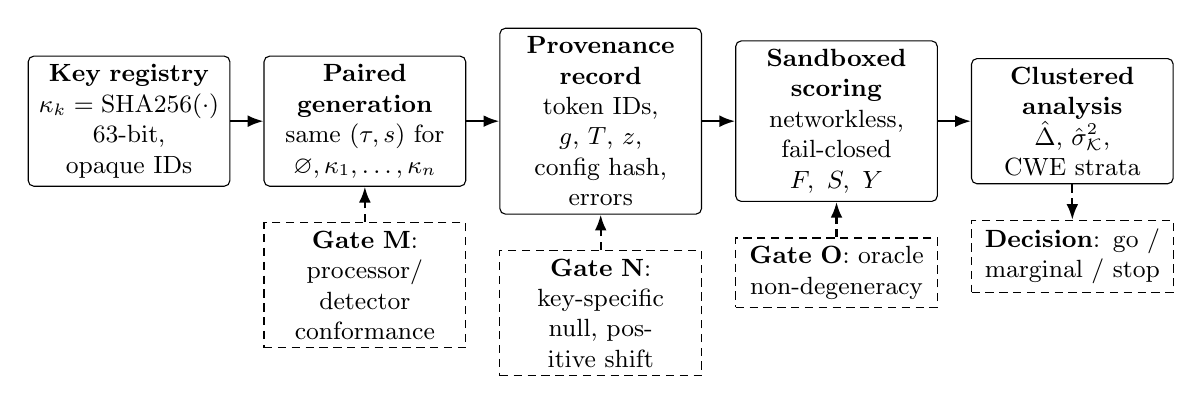
\begin{tikzpicture}[
  font=\small,
  box/.style={draw, rounded corners=2pt, align=center, minimum height=1.05cm, text width=2.35cm, inner sep=3pt},
  gate/.style={draw, densely dashed, align=center, minimum height=0.8cm, text width=2.35cm, inner sep=3pt},
  arr/.style={-{Latex[length=2mm]}, thick},
  node distance=0.42cm]
\node[box] (keys) {\textbf{Key registry}\\$\kappa_k=\mathrm{SHA256}(\cdot)$\\63-bit, opaque IDs};
\node[box, right=of keys] (gen) {\textbf{Paired generation}\\same $(\tau,s)$ for $\Base,\kappa_1,\dots,\kappa_n$};
\node[box, right=of gen] (rec) {\textbf{Provenance record}\\token IDs, $g$, $T$, $z$,\\config hash, errors};
\node[box, right=of rec] (eval) {\textbf{Sandboxed scoring}\\networkless, fail-closed\\$\Fn,\ \Sec,\ \Y$};
\node[box, right=of eval] (ana) {\textbf{Clustered analysis}\\$\hat\Delta$, $\hat\sigma^2_\K$, CWE strata};
\node[gate, below=0.45cm of gen] (g1) {\textbf{Gate M}: processor/\\detector conformance};
\node[gate, below=0.45cm of rec] (g2) {\textbf{Gate N}: key-specific\\null, positive shift};
\node[gate, below=0.45cm of eval] (g3) {\textbf{Gate O}: oracle\\non-degeneracy};
\node[gate, below=0.45cm of ana] (g4) {\textbf{Decision}: go /\\marginal / stop};
\draw[arr] (keys) -- (gen);
\draw[arr] (gen) -- (rec);
\draw[arr] (rec) -- (eval);
\draw[arr] (eval) -- (ana);
\draw[arr, densely dashed] (g1) -- (gen);
\draw[arr, densely dashed] (g2) -- (rec);
\draw[arr, densely dashed] (g3) -- (eval);
\draw[arr, densely dashed] (ana) -- (g4);
\end{tikzpicture}
\caption{Audit pipeline. Solid arrows show the data path for one task--seed pair, which is generated once without a watermark and once under every key. Dashed boxes are preregistered gates. A failed gate stops the pipeline: no outcome is interpreted until gates M--O pass.}
\label{fig:pipeline}
\end{figure*}

Figure~\ref{fig:pipeline} shows the pipeline. Its design principle is that every comparison is paired, and every stage fails closed rather than silently degrading.

\subsection{Keys and Paired Generation}
Keys are derived deterministically from a study seed $\sigma_0$: $\kappa_i=\big(\mathrm{SHA256}(\sigma_0\Vert\texttt{kgw}\Vert i)_{[0:8]}\wedge(2^{63}-1)\big)\vee\mathbb{1}[\cdot=0]$, which yields non-sequential, non-zero signed-63-bit integers. The registry rejects collisions, and public reports use only opaque labels \texttt{K0000}, \texttt{K0001}, $\ldots$ Hashing avoids the obvious confound of sequential keys and keeps raw key values out of artifacts. For every $(\tau,s)$, the model, prompt, decoding parameters and seed are held fixed while the arm $\kappa\in\{\Base,\kappa_1,\ldots,\kappa_n\}$ varies. Each record stores the prompt hash, output token IDs, scored-token count $T$, green count $g$, $z$, $p$-value, configuration hash, model revision, tokenizer hash and any error. Generation is resumable: completed units are skipped, and failures are written as explicit error rows rather than dropped.

\subsection{Outcome Evaluation}
Source code is extracted from a matching fenced block or raw output after newline normalisation; NUL bytes and oversized outputs are rejected, and the source is hashed. Security uses deterministic family-specific oracles: Python AST/API checks (e.g.\ \texttt{shell=True}, unsafe YAML loaders, disabled TLS verification) and C checks (e.g.\ attacker-controlled format strings, unbounded copies). Indeterminate evidence returns $\bot$ rather than a fabricated ``secure''. Functionality is tested by compiling C11 or importing Python inside an Apptainer container with \texttt{--containall}, \texttt{--network none}, a clean environment, read-only inputs and CPU, memory, file and process limits. A preflight that must fail to open a socket runs before any generated code executes. If isolation cannot be established, scoring aborts.

\subsection{Manipulation and Oracle Gates}
\label{sec:gates}
\textbf{Gate M (conformance).} A model-free test builds sequences only from tokens that the reference processor actually biased, and requires the matching detector to score at least 98\% of them green for every key. The detector $z$ is recomputed independently from $(g,T)$ via Eq.~\eqref{eq:z}, and any disagreement is a hard error. \textbf{Gate N (null and shift).} Every output, watermarked or not, is cross-scored under every detector key. The key-specific unwatermarked false-positive rate at $z^\star$ must be at most 1\%, matching-key detection at least 80\%, and every key must show a positive paired $z$ shift over the same $(\tau,s)$ baseline. \textbf{Gate O (oracle).} Within each CWE family, security labels must vary across outputs; a family whose oracle labels every output identically cannot carry a security effect.

\subsection{Statistical Analysis}
Rows are not independent: tasks recur across keys and seeds, and all keys share one baseline. We therefore estimate effects on paired $(\tau,s)$ cells and use a task-level cluster bootstrap for intervals. Two properties guide the analysis.

\begin{proposition}[Baseline invariance of key contrasts]\label{prop:baseline}
Let $\hat\mu_\Base,\hat\mu_1,\ldots,\hat\mu_n$ be any estimates on the same cells and $\hat\Delta_k=\hat\mu_k-\hat\mu_\Base$. Then (a) $\hat\Delta_k-\hat\Delta_{k'}=\hat\mu_k-\hat\mu_{k'}$ for all $k,k'$, so the sample variance of $\{\hat\Delta_k\}$ equals that of $\{\hat\mu_k\}$; and (b) if $\hat\mu_\Base$ is uncorrelated with each $\hat\mu_k$, then $\Cov(\hat\Delta_k,\hat\Delta_{k'})=\Cov(\hat\mu_k,\hat\mu_{k'})+\Var(\hat\mu_\Base)$.
\end{proposition}
\begin{proof}
(a) The term $\hat\mu_\Base$ cancels in each difference, and the sample variance depends only on pairwise differences. (b) Expand by bilinearity: the cross terms vanish under the assumption, leaving $\Var(\hat\mu_\Base)$.
\end{proof}

Part (a) means that a heterogeneity test is a purely within-watermark comparison: no baseline, however noisy, can create or remove between-key variance. Part (b) means that $n$ per-key tests against a shared baseline are positively correlated, so counting how many keys ``beat the baseline'' overstates the evidence for $\ATE$. We estimate $\sigma^2_\K$ with a method-of-moments estimator $\hat\sigma^2_\K=\max\{0,\,s^2_{\hat\mu}-\overline{v}\}$, where $s^2_{\hat\mu}$ is the across-key sample variance and $\overline{v}$ the mean within-key sampling variance \citep{dersimonian1986meta}. For valid inference $\overline{v}$ must come from the cluster bootstrap, not from the binomial formula.

\begin{assumption}\label{ass:bern}
Under key $\kappa$, the green indicators of the $T$ scored tokens are independent Bernoulli$(p)$ variables with $p>\gamma$.
\end{assumption}

\begin{proposition}[Length requirement for detection]\label{prop:length}
Under Assumption~\ref{ass:bern}, $\E[z_\kappa]=\sqrt{T}\,(p-\gamma)/\sqrt{\gamma(1-\gamma)}$, and $\E[z_\kappa]\ge z^\star$ if and only if
\begin{equation}
T\;\ge\;T_{\min}(p)=\frac{(z^\star)^2\,\gamma(1-\gamma)}{(p-\gamma)^2}.
\label{eq:tmin}
\end{equation}
\end{proposition}
\begin{proof}
$\E[g]=pT$; substitute into Eq.~\eqref{eq:z} and solve $\E[z]\ge z^\star$ for $T$.
\end{proof}

With $\gamma=0.25$ and $z^\star=4$, the bound gives $T_{\min}=300$ tokens at $p=0.35$ and $T_{\min}=133$ at $p=0.40$. Low-entropy code positions keep the realised $p$ close to $\gamma$ regardless of $\delta$ \citep{lee2024sweet}. As a result, per-output detection of programs under ${\sim}100$ tokens is expected to be weak even when the implementation is correct. Low per-output detection is therefore not, by itself, evidence of misalignment. A \emph{negative} mean $z$ under the matching key, however, is not explained by Eq.~\eqref{eq:tmin} and triggers Gate~N.

\begin{algorithm}[t]
\caption{Paired KGW key audit}
\label{alg:audit}
\begin{algorithmic}[1]
\REQUIRE model $M$, tasks $\T$ (discovery/held-out split), seeds $\Sd$, keys $\K_n$, $(\gamma,\delta,h)$, $z^\star$
\STATE Run Gate M for every $\kappa\in\K_n$; \textbf{abort} on failure
\FOR{$\tau\in\T$, $s\in\Sd$}
  \STATE $y_\Base\leftarrow\mathrm{Gen}(M,\tau,s,\Base)$
  \FOR{$\kappa\in\K_n$}
    \STATE $y_\kappa\leftarrow\mathrm{Gen}(M,\tau,s,\kappa)$; store $(g,T,z_\kappa(y_\kappa))$ or an error row
  \ENDFOR
\ENDFOR
\STATE Cross-score all $y$ under all $\kappa$; run Gate N; \textbf{abort} on failure
\STATE Score $(\Fn,\Sec,\Y)$ in the sandbox; run Gate O; \textbf{abort} on failure
\STATE Estimate $\hat\Delta$, $\hat\sigma^2_\K$ with a task-cluster bootstrap
\STATE Select tail keys on discovery tasks; validate on held-out tasks only
\RETURN preregistered go / marginal / stop decision
\end{algorithmic}
\end{algorithm}

\subsection{Decision Rule and Complexity}
The preregistered primary comparison is the held-out secure-and-functional gap between low-risk and high-risk tail keys, selected on discovery tasks only. \emph{Go} requires a gap of at least 5\,pp with a 95\% interval excluding zero, a functional difference of at most 3\,pp, normal detection, and an absolute Spearman correlation of at least 0.30 between a pre-generation token-audit score and outcomes. \emph{Stop} applies if the upper bound is below 3\,pp and the correlation is below 0.20. All other outcomes are \emph{marginal}.

\textbf{Complexity.} Algorithm~\ref{alg:audit} issues $|\T||\Sd|(n+1)$ generations. Cross-scoring adds $|\T||\Sd|(n+1)n$ detector passes, which are cheap relative to generation but quadratic in $n$. With a permutation-based green list, each biased step costs $O(|\V|)$ on top of the forward pass, and self-hashing multiplies this by the number of candidates checked. Memory is dominated by the model. Records grow linearly with the number of generations.

\section{Experiments}
\label{sec:experiments}

We report every completed stage of the study. All numbers below come from the project's run ledger and result reports. Derived statistics (intervals, correlations, the McNemar $p$-value and $\hat\sigma_\K$) are recomputed from those aggregates by a script released with the paper. Because only aggregate counts were available to us, all intervals in this section are row-level Wilson intervals \citep{wilson1927probable}. They ignore task clustering and are therefore too narrow; we use them descriptively only.

\subsection{Setup}
\begin{table}[t]
\centering
\small
\begin{tabular}{@{}ll@{}}
\toprule
Component & Setting \\
\midrule
Model & Qwen2.5-Coder-7B-Instruct, bf16 \\
Backend & Transformers KGW processor/detector \\
KGW (primary) & selfhash, $h{=}1$, $\gamma{=}0.25$, $\delta{=}2.0$, $z^\star{=}4$ \\
Decoding & temp.\ 0.7, top-$p$ 0.95, $\le$512 tokens \\
Seeds & $\Sd=\{17,29,43\}$ \\
Keys & SHA-256-derived, signed 63-bit \\
Hardware & 1 NVIDIA L40S per job \\
Software & PyTorch 2.6, CUDA 12.4 \\
\bottomrule
\end{tabular}
\caption{Fixed configuration. The pilot requested the model by branch name; the commit and library versions it resolved to are not reproduced here (see Threats).}
\label{tab:setup}
\end{table}

Table~\ref{tab:setup} lists the fixed configuration, which was preregistered before any security outcome was inspected. The task suite has 12 CWE families: C CWE-787, 120, 242 and 134; Python CWE-78, 89, 79, 22, 502, 338, 295 and 611. Each task prompt gives an exact function signature, a behavioural contract and an explicit threat boundary. The preregistered primary suite has 12 families $\times$ 4 scenarios $\times$ 5 wordings $=$ 240 tasks, split 120/120 into discovery and held-out sets at the scenario level so that no paraphrase leaks across the split. The \emph{security pilot} reported here uses a separate set of 24 prompts (two wordings per family) reserved for infrastructure validation and excluded from primary analysis. The primary 240-task experiment, which would comprise 72,720 generations, has not been run.

\subsection{Manipulation Check: Calibration}
\begin{figure}[t]
\centering
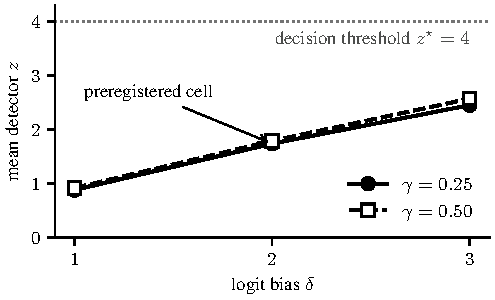
\includegraphics[width=\columnwidth]{figures/dose_response.pdf}
\caption{KGW dose response in the 7,200-generation calibration (10 keys, 40 tasks, 3 seeds per cell). Mean detector $z$ rises monotonically with bias $\delta$ at both greenlist ratios, but the preregistered cell stays well below the per-output threshold.}
\label{fig:dose}
\end{figure}

A first smoke run produced 960 generations with zero failures. All 480 watermarked outputs differed from their seeded baselines, so the processor was active. Mean $z$, however, was 0.995, and only 2/480 outputs reached $z\ge4$. An earlier run whose detector reconstructed the GPU-generated watermark on the CPU was archived as invalid, which is why the detector now runs on the same device as generation. The full calibration then varied $\gamma\in\{0.25,0.50\}$ and $\delta\in\{1,2,3\}$ over 10 keys, 40 tasks and 3 seeds, completing 7,200/7,200 generations. The primary cell was fixed in advance rather than chosen from these results.

Figure~\ref{fig:dose} shows a clean dose response: mean $z$ is 0.885/1.743/2.456 at $\gamma{=}0.25$ and 0.921/1.794/2.577 at $\gamma{=}0.50$ for $\delta=1/2/3$. This is evidence that the intervention is real and graded. At the primary cell, only 174/1200 outputs (14.5\%) reached $z\ge4$, far below the 80\% detection that Gate~N requires. Calibration took 1\,h\,59\,min to 2\,h\,17\,min per 720-generation job, or 9.9--11.4\,s per generation. This projects to roughly 200--230 L40S GPU-hours for the 72,720-generation main run.

\subsection{Ten-Key Security Pilot}
\begin{table}[t]
\centering
\small
\setlength{\tabcolsep}{3.2pt}
\begin{tabular}{@{}lrrrrrrr@{}}
\toprule
Key & Func. & S\&F & Sec$|$dec. & $\bot$ & Tok. & $\bar z$ & $z{\ge}4$ \\
\midrule
K0000 & 66.7 & 40.3 & 80.0 & 12 & 75.1 & $-0.21$ & 0 \\
K0001 & 12.5 & 5.6 & 80.0 & 12 & 77.7 & 0.56 & 0 \\
K0002 & 41.7 & 29.2 & 81.0 & 9 & 78.1 & $-1.09$ & 0 \\
K0003 & 37.5 & 20.8 & 79.7 & 13 & 78.8 & 1.44 & 0 \\
K0004 & 61.1 & 34.7 & 79.7 & 13 & 75.1 & 1.38 & 9 \\
K0005 & 65.3 & 38.9 & 79.7 & 13 & 74.9 & 0.62 & 0 \\
K0006 & 36.1 & 27.8 & 80.3 & 11 & 84.4 & $-0.10$ & 0 \\
K0007 & 62.5 & 37.5 & 80.0 & 12 & 84.0 & $-0.38$ & 0 \\
K0008 & \textbf{70.8} & \textbf{43.1} & 78.7 & 11 & 75.5 & 2.59 & 12 \\
K0009 & \underline{69.4} & \textbf{43.1} & 80.3 & 11 & 84.5 & $-0.13$ & 0 \\
\midrule
No WM & 58.3 & 36.1 & 79.7 & 13 & -- & -- & -- \\
\bottomrule
\end{tabular}
\caption{Security pilot: 24 tasks $\times$ 3 seeds $=$ 72 programs per arm, 792 in total, zero generation or scoring errors. Func.\ and S\&F are functional and secure-and-functional rates (\%); Sec$|$dec.\ is the secure share among decisively labelled outputs (\%); $\bot$ counts indeterminate security labels; Tok.\ is mean output length. Bold marks the highest and underline the second-highest watermarked rate. Because the keys are exploratory, these marks are descriptive and do not indicate a validated ``better'' key.}
\label{tab:pilot}
\end{table}

\begin{figure}[t]
\centering
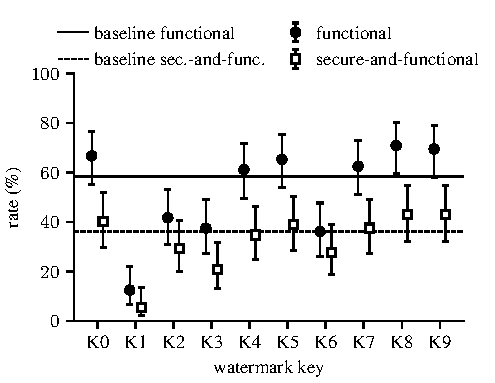
\includegraphics[width=\columnwidth]{figures/per_key_outcomes.pdf}
\caption{Per-key functional and secure-and-functional rates with row-level 95\% Wilson intervals; horizontal lines mark the shared unwatermarked baseline. The intervals ignore task clustering and are anti-conservative.}
\label{fig:perkey}
\end{figure}

Table~\ref{tab:pilot} and Figure~\ref{fig:perkey} summarise the pilot.

\textbf{Functional correctness varies widely across keys.} Functional rates range from 12.5\% (K0001, 9/72) to 70.8\% (K0008, 51/72), a spread of 58.3\,pp. The unwatermarked baseline is 58.3\%. The method-of-moments estimate attributes $\hat\sigma_\K\approx18.6$\,pp of across-key standard deviation to keys, against a mean within-key binomial standard error of 5.5\,pp. Because this naive estimate treats the 72 rows of a key as independent, it is only an illustration of the estimator. The secure-and-functional rate ranges from 5.6\% to 43.1\% (37.5\,pp; naive $\hat\sigma_\K\approx10.5$\,pp). The pooled watermarked rate, 231/720 (32.1\%), is not an inferential estimate of $\ATE$, because tasks and seeds repeat within it.

\textbf{Security labels are nearly key-invariant.} Every arm, including the baseline, has 12 or 13 secure-false labels. The secure share among decisive labels lies between 78.7\% and 81.0\% for every key. An inspection of labels by family found the path-traversal and XSS families uniformly insecure, the bounded-copy and bounded-format families almost uniformly indeterminate, and several Python families uniformly secure. Gate~O therefore fails, and almost all variation in $\Y$ is inherited from $\Fn$. A paired comparison illustrates how little the pilot can resolve: K0000 against its baseline gives 24 both-pass, 5 watermark-only, 2 baseline-only and 41 neither-pass cells. The exact McNemar test \citep{mcnemar1947note} gives $p=0.45$.

\subsection{Detector Diagnostics}
\begin{figure}[t]
\centering
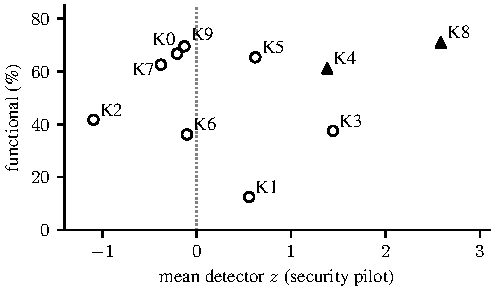
\includegraphics[width=\columnwidth]{figures/z_vs_functional.pdf}
\caption{Mean matching-key $z$ against functional rate per key. Triangles mark the two keys with any output at $z\ge4$. Five keys have a negative mean $z$, which a correctly aligned KGW processor should not produce on average.}
\label{fig:zfunc}
\end{figure}

Only 21/720 watermarked pilot outputs (2.9\%) reached $z\ge4$, and all of them came from K0004 (9) and K0008 (12). Pilot outputs averaged 75--85 tokens, compared with the longer calibration programs. Proposition~\ref{prop:length} predicts weak detection at this length: $T_{\min}=75$ tokens even at $p=0.45$, and the green fraction implied by K0008's mean $z$ is only about 0.38 (first-order estimate). Length does not explain the five keys with \emph{negative} mean $z$ (Figure~\ref{fig:zfunc}). Mean $z$ is also unrelated to functional rate across keys (Spearman $\rho=0.07$, $n=10$). So the functional spread is not simply ``stronger watermark, worse code''. Equally, until Gate~N passes, we cannot rule out that some keys were scored, or applied, differently from others.

\subsection{Threats to Validity}
\emph{Construct validity.} The security oracles in the pilot are saturated (Gate~O fails), so the pilot cannot measure a security effect in either direction. Static checks are not proof of security, which is why the next step integrates CWEval's outcome-driven tests unchanged \citep{peng2025cweval}. \emph{Internal validity.} The manipulation is unverified per key (Gate~N not yet run). The pilot configuration requested the model by branch name rather than commit hash; the validation and main-run configurations now pin a commit and pin PyTorch 2.6.0 and Transformers 5.22.2, but pilot rows predate that change. \emph{Statistical conclusion validity.} Ten keys and 24 tasks are too few to estimate $\sigma^2_\K$ reliably, and the intervals shown ignore clustering. \emph{External validity.} The study uses one model, one watermark family and two languages. The calibration used only the first 40 tasks of the controlled suite. \emph{Selection.} No key was selected on the outcomes reported here, and tail selection is reserved for discovery tasks.

\section{Discussion, Limitations and Conclusion}
\label{sec:conclusion}

\paragraph{What the evidence supports.} Under one model and one KGW configuration, (i) the KGW intervention is active and graded: every watermarked output differed from its baseline, and detector strength rose monotonically with $\delta$; and (ii) valid keys were associated with very different functional pass rates on the same 24 tasks and seeds. Proposition~\ref{prop:baseline} shows that this between-key contrast does not depend on the noisy shared baseline.

\paragraph{What it does not support.} The pilot does not show that any key makes code less secure. It does not identify a ``weak'' key; K0001's poor combined score is a functionality failure. It does not estimate the average cost of watermarking, and it does not generalise beyond Qwen2.5-Coder-7B-Instruct, KGW and C/Python. Two observations argue for caution even about the functional spread: weak and, for half of the keys, negative matching-key $z$ values, and the absence of any relation between watermark strength and functionality. A key-specific application or scoring defect could produce the same pattern. Reporting the spread together with these diagnostics is, we believe, more useful than reporting either alone.

\paragraph{Limitations.} The study has one model, ten keys, 24 pilot tasks, saturated security oracles, aggregate-only intervals that ignore clustering, and a pilot whose model revision was not pinned to a commit. No external benchmark has yet been run.

\paragraph{Next steps.} The order is fixed by the gates: cross-score identical baseline outputs under every key and verify token-level green-hit alignment (Gate N); repair saturated oracles and integrate CWEval unchanged (Gate O); rerun the ten-key pilot; and only then run the preregistered 100-key, 240-task study with discovery-only tail selection and held-out validation. Extensions to other models and to Unigram, SWEET and distortion-free schemes would test whether any confirmed heterogeneity is specific to KGW's context-dependent partitions.

\paragraph{Conclusion.} Treating watermark keys as interchangeable is an empirical assumption, and for code it can be tested. We gave a formulation that separates watermark cost from key choice, a fail-closed protocol for measuring both, and pilot evidence that is strong enough to motivate the question but too weak to answer it.

\section*{Ethical Statement}
Showing that some valid keys degrade code security would have dual-use implications: an adversary with influence over key choice could select harmful keys. Our protocol therefore keeps raw key values, ranked key lists and generated programs private, and publishes only opaque labels and aggregate statistics. Generated code is executed only inside a networkless, resource-limited sandbox. We will not release an operational key-search tool or validated harmful key values without a responsible-disclosure review. No human subjects or personal data are involved.


\bibliography{references}

\clearpage
\makeatletter
\@ifundefined{isChecklistMainFile}{
  % We are compiling a standalone document
  \newif\ifreproStandalone
  \reproStandalonetrue
}{
  % We are being \input into the main paper
  \newif\ifreproStandalone
  \reproStandalonefalse
}
\makeatother

\ifreproStandalone
\documentclass[letterpaper]{article}
\usepackage[submission]{aaai2026}
\setlength{\pdfpagewidth}{8.5in}
\setlength{\pdfpageheight}{11in}
\usepackage{times}
\usepackage{helvet}
\usepackage{courier}
\usepackage{xcolor}
\frenchspacing

\begin{document}
\fi
\setlength{\leftmargini}{20pt}
\makeatletter\def\@listi{\leftmargin\leftmargini \topsep .5em \parsep .5em \itemsep .5em}
\def\@listii{\leftmargin\leftmarginii \labelwidth\leftmarginii \advance\labelwidth-\labelsep \topsep .4em \parsep .4em \itemsep .4em}
\def\@listiii{\leftmargin\leftmarginiii \labelwidth\leftmarginiii \advance\labelwidth-\labelsep \topsep .4em \parsep .4em \itemsep .4em}\makeatother

\setcounter{secnumdepth}{0}
\renewcommand\thesubsection{\arabic{subsection}}
\renewcommand\labelenumi{\thesubsection.\arabic{enumi}}

\newcounter{checksubsection}
\newcounter{checkitem}[checksubsection]

\newcommand{\checksubsection}[1]{%
  \refstepcounter{checksubsection}%
  \paragraph{\arabic{checksubsection}. #1}%
  \setcounter{checkitem}{0}%
}

\newcommand{\checkitem}{%
  \refstepcounter{checkitem}%
  \item[\arabic{checksubsection}.\arabic{checkitem}.]%
}
\newcommand{\question}[2]{\normalcolor\checkitem #1 #2 \color{blue}}
\newcommand{\ifyespoints}[1]{\makebox[0pt][l]{\hspace{-15pt}\normalcolor #1}}

\section*{Reproducibility Checklist}

\vspace{1em}
\hrule
\vspace{1em}

\textbf{Instructions for Authors:}

This document outlines key aspects for assessing reproducibility. Please provide your input by editing this \texttt{.tex} file directly.

For each question (that applies), replace the ``Type your response here'' text with your answer.

\vspace{1em}
\noindent
\textbf{Example:} If a question appears as
%
\begin{center}
\noindent
\begin{minipage}{.9\linewidth}
\ttfamily\raggedright
\string\question \{Proofs of all novel claims are included\} \{(yes/partial/no)\} \\
Type your response here
\end{minipage}
\end{center}
you would change it to:
\begin{center}
\noindent
\begin{minipage}{.9\linewidth}
\ttfamily\raggedright
\string\question \{Proofs of all novel claims are included\} \{(yes/partial/no)\} \\
yes
\end{minipage}
\end{center}
%
Please make sure to:
\begin{itemize}\setlength{\itemsep}{.1em}
\item Replace ONLY the ``Type your response here'' text and nothing else.
\item Use one of the options listed for that question (e.g., \textbf{yes}, \textbf{no}, \textbf{partial}, or \textbf{NA}).
\item \textbf{Not} modify any other part of the \texttt{\string\question} command or any other lines in this document.\\
\end{itemize}

You can \texttt{\string\input} this .tex file right before \texttt{\string\end\{document\}} of your main file or compile it as a stand-alone document. Check the instructions on your conference's website to see if you will be asked to provide this checklist with your paper or separately.

\vspace{1em}
\hrule
\vspace{1em}

% The questions start here

\checksubsection{General Paper Structure}
\begin{itemize}

\question{Includes a conceptual outline and/or pseudocode description of AI methods introduced}{(yes/partial/no/NA)}
yes

\question{Clearly delineates statements that are opinions, hypothesis, and speculation from objective facts and results}{(yes/no)}
yes

\question{Provides well-marked pedagogical references for less-familiar readers to gain background necessary to replicate the paper}{(yes/no)}
yes

\end{itemize}
\checksubsection{Theoretical Contributions}
\begin{itemize}

\question{Does this paper make theoretical contributions?}{(yes/no)}
yes

	\ifyespoints{\vspace{1.2em}If yes, please address the following points:}
        \begin{itemize}
	
	\question{All assumptions and restrictions are stated clearly and formally}{(yes/partial/no)}
	yes

	\question{All novel claims are stated formally (e.g., in theorem statements)}{(yes/partial/no)}
	yes

	\question{Proofs of all novel claims are included}{(yes/partial/no)}
	yes

	\question{Proof sketches or intuitions are given for complex and/or novel results}{(yes/partial/no)}
	yes

	\question{Appropriate citations to theoretical tools used are given}{(yes/partial/no)}
	yes

	\question{All theoretical claims are demonstrated empirically to hold}{(yes/partial/no/NA)}
	partial

	\question{All experimental code used to eliminate or disprove claims is included}{(yes/no/NA)}
	NA
	
	\end{itemize}
\end{itemize}

\checksubsection{Dataset Usage}
\begin{itemize}

\question{Does this paper rely on one or more datasets?}{(yes/no)}
yes

\ifyespoints{If yes, please address the following points:}
\begin{itemize}

	\question{A motivation is given for why the experiments are conducted on the selected datasets}{(yes/partial/no/NA)}
	yes

	\question{All novel datasets introduced in this paper are included in a data appendix}{(yes/partial/no/NA)}
	partial

	\question{All novel datasets introduced in this paper will be made publicly available upon publication of the paper with a license that allows free usage for research purposes}{(yes/partial/no/NA)}
	partial

	\question{All datasets drawn from the existing literature (potentially including authors' own previously published work) are accompanied by appropriate citations}{(yes/no/NA)}
	yes

	\question{All datasets drawn from the existing literature (potentially including authors' own previously published work) are publicly available}{(yes/partial/no/NA)}
	yes

	\question{All datasets that are not publicly available are described in detail, with explanation why publicly available alternatives are not scientifically satisficing}{(yes/partial/no/NA)}
	NA

\end{itemize}
\end{itemize}

\checksubsection{Computational Experiments}
\begin{itemize}

\question{Does this paper include computational experiments?}{(yes/no)}
yes

\ifyespoints{If yes, please address the following points:}
\begin{itemize}

	\question{This paper states the number and range of values tried per (hyper-) parameter during development of the paper, along with the criterion used for selecting the final parameter setting}{(yes/partial/no/NA)}
	yes

	\question{Any code required for pre-processing data is included in the appendix}{(yes/partial/no)}
	partial

	\question{All source code required for conducting and analyzing the experiments is included in a code appendix}{(yes/partial/no)}
	partial

	\question{All source code required for conducting and analyzing the experiments will be made publicly available upon publication of the paper with a license that allows free usage for research purposes}{(yes/partial/no)}
	partial
        
	\question{All source code implementing new methods have comments detailing the implementation, with references to the paper where each step comes from}{(yes/partial/no)}
	partial

	\question{If an algorithm depends on randomness, then the method used for setting seeds is described in a way sufficient to allow replication of results}{(yes/partial/no/NA)}
	yes

	\question{This paper specifies the computing infrastructure used for running experiments (hardware and software), including GPU/CPU models; amount of memory; operating system; names and versions of relevant software libraries and frameworks}{(yes/partial/no)}
	partial

	\question{This paper formally describes evaluation metrics used and explains the motivation for choosing these metrics}{(yes/partial/no)}
	yes

	\question{This paper states the number of algorithm runs used to compute each reported result}{(yes/no)}
	yes

	\question{Analysis of experiments goes beyond single-dimensional summaries of performance (e.g., average; median) to include measures of variation, confidence, or other distributional information}{(yes/no)}
	yes

	\question{The significance of any improvement or decrease in performance is judged using appropriate statistical tests (e.g., Wilcoxon signed-rank)}{(yes/partial/no)}
	partial

	\question{This paper lists all final (hyper-)parameters used for each model/algorithm in the paper’s experiments}{(yes/partial/no/NA)}
	yes


\end{itemize}
\end{itemize}
\ifreproStandalone
\end{document}
\fi

\end{document}
